\documentclass[11pt,a4paper]{article}
\usepackage[utf8]{inputenc}
\usepackage[english]{babel}
\usepackage{amsmath}
\usepackage{amsfonts}
\usepackage{amssymb}
\usepackage{graphicx}
\usepackage{multicol}
\usepackage{pifont} % Check mark and cross mark
\usepackage[left=2cm,right=2cm,top=1.5cm,bottom=2cm]{geometry}

\newcommand\independent{\protect\mathpalette{\protect\independenT}{\perp}}
\def\independenT#1#2{\mathrel{\rlap{$#1#2$}\mkern2mu{#1#2}}}

\newcommand{\cmark}{\ding{51}}%
\newcommand{\xmark}{\ding{55}}%

\begin{document}
\begin{center}
{\Large Probabilistic Modelling and Reasoning: Assignment}\\
{\large UNN: S1796157}
\end{center}

\section*{Question 1}

\subsection*{a-c)}

\begin{multicols}{3}
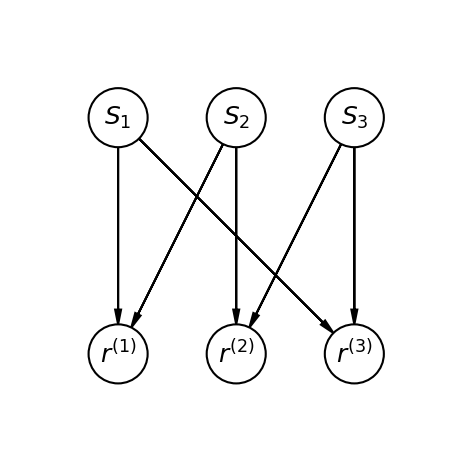
\includegraphics[scale=0.6]{./images/q1a.png}
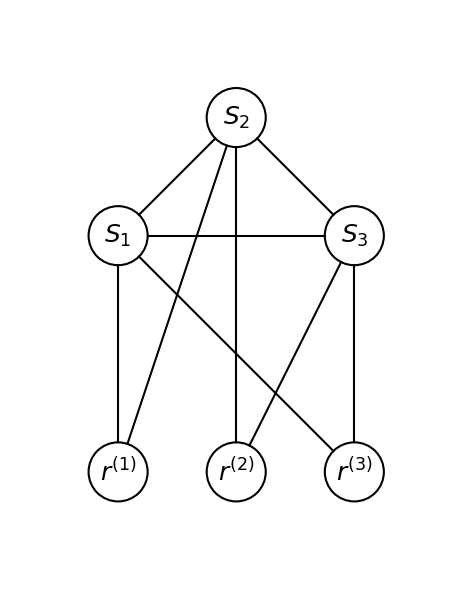
\includegraphics[scale=0.6]{./images/q1c.png}
These graphs show the solutions to question $a$ and question $c$.
On the left side we have the DGM and on the right side we have the
undirected minimal I-map generatet from the DGM.
\end{multicols}


\subsection*{b)}
\begin{itemize}
\item $s_1 \bot s_2 \; | \; r^{(2)}$. This independence assertion holds since all trails from
$s_1$ and $s_2$ are blocked;
\item $s_1 \bot s_2 \; | \; r^{(3)}, r^{(2)}$. This independence assertion does not hold since
there is a trail between $s_1$ and $s_2$ which is not blocked, namely $s_1 \rightarrow r^{(3)} \rightarrow s_3
\rightarrow r^{(2)} \rightarrow s_2$.
\end{itemize}

\subsection*{d)}
\begin{table}[h]
\begin{tabular}{p{3.5cm}ccp{10cm}}
\hline
\multicolumn{1}{|p{3.5cm}|}{\textbf{Independence}} & \multicolumn{1}{c|}{\textbf{DGM}} & \multicolumn{1}{c|}{\textbf{UGM}} & \multicolumn{1}{c|}{\textbf{Justification}} \\ \hline
$s_1 \independent r^{2} \; | \; \{s_2, s_3\}$ & \cmark & \cmark & DGM: cond. on $s_2$ and $s_3$ blocks all path from $s_1$.
\smallskip

UGM: cond. on $s_2$ and $s_3$ blocks all path between $s_1$ and $r^{(2)}$. \\
$s_1 \independent r^{2} \; | \; \{ r^{(1)}, s_3 \} $ & \xmark & \xmark & DGM: path not blocked $s_1 \rightarrow r^{(1)} \rightarrow s_2 \rightarrow r^{(2)} $.
\smallskip

UGM: path not blocked $s_1 \rightarrow s_3 \rightarrow r^{2}$. 
\\
$ s_1 \independent s_2 $ & \cmark & \xmark & DGM: connected head-to-head with no evidence on $r^{(1)}$, hence trail blocked.
\smallskip

UGM: hence the independence relation does not hold..\\
$ s_1 \independent s_2 \; | \; \{ r^{(1)} \}$&\xmark &\xmark & DGM: path not blocked $s_1 \rightarrow r^{(1)} \rightarrow s_2$.
\smallskip

UGM: $s_1$ and $s_2$ are connected directly, hence the independence relation does not hold.\\
$r^{(1)} \independent r^{(2)}$& \xmark & \xmark & DGM: connected tail-to-tail with no evidence on $s_2$.
\smallskip

UGM: there are many open paths between $r_{(1)}$ and $r^{(2)}$.
\\
$r^{(1)} \independent r^{(2)} \; | \; \{ s_2 \}$& \cmark & \xmark & DGM: all path between $r^{(1)}$ and $r^{(2)}$ are blocked.
\smallskip

UGM: cond. on $s_2$ leaves many open paths between $r_{(1)}$ and $r^{(2)}$.
\\
$r^{(1)} \independent r^{(2)} \; | \; \{ s_1, s_2 \}$ & \cmark & \cmark & DGM: all path between $r^{(1)}$ and $r^{(2)}$ are blocked.
\smallskip

UGM: cond. on $s_1$ and $s_2$ blocks all paths.
\\
$r^{(1)} \independent r^{(2)} \; | \; \{ s_2, r^{3} \}$&\xmark & \xmark& DGM: open path between $r^{(1)}$ and $r^{(2)}$, namely $r^{(1)} \rightarrow s_1 \rightarrow r^{(3)} \rightarrow s_3 \rightarrow r^{(2)}$.
\smallskip

UGM: cond. on $s_2$ and $r^\{(3)\}$ leaves many open paths. \\
\end{tabular}
\end{table}

\section*{Question 2}

\subsection*{a)}
The factorization of the pmf over the graph showed in the answer $a$ of question1 is given by the formula showed below, in which $pa_i$ represents the parents of the variable $x_i$ in the graph:
\begin{equation}
\mathbb{P}(x_1, \ldots, x_n) = \prod_{i=1}^{n} \mathbb{P}[x_i \; | \; pa_i]
\end{equation}
Therefore, the pmf for $\mathbb{P}[s_1, s_2, s_3, r^{(1)}, r^{(2)}, r^{(3)}]$ becomes:
\begin{equation}
\mathbb{P}[s_1, s_2, s_3, r^{(1)}, r^{(2)}, r^{(3)}] = \mathbb{P}[r^{1} \; | \; s_1, s_2]\cdot \mathbb{P}[r^{2} \; | \; s_2, s_3] \cdot \mathbb{P}[r^{3} \; | \; s_1, s_3] \cdot \mathbb{P}[s_1] \cdot \mathbb{P}[s_2] \cdot \mathbb{P}[s_3]
\end{equation}

\subsection*{b)}
\begin{itemize}
\item $\phi_1(s_1)$
\item $\phi_2(s_2)$
\item $\phi_3(s_3)$
\item $\phi_A(s_1, s_2, r^{(1)})$
\item $\phi_B(s_2, s_3, r^{(2)})$
\item $\phi_C(s_1, s_3, r^{(3)})$
\end{itemize}

\subsection*{c}

\end{document}